\documentclass{beamer}

%\usepackage[style=authortitle,backend=bibtex]{biblatex}
%\addbibresource{source.bib}
\usepackage{wasysym}
\usepackage[center]{caption}

% === ENCODINGS === 

\usepackage[english, russian]{babel}
\usepackage[T2A]{fontenc}
\usepackage[utf8]{inputenc}

% === MATH === 

% Some math fonts
\usepackage{amsfonts}

% Some math symbols
\usepackage{amssymb}

% Some math "making beautiful" stuff
\usepackage{mathtools}

% Some math fonts
\usepackage{mathrsfs}  

\numberwithin{equation}{section}

% === REFERENCES ===

\usepackage[sorting=none]{biblatex}
\addbibresource{sources.bib}


% === MY COMMANDS ===

\newcommand{\deriv}[2]{\frac{\partial #1}{\partial #2}}
\newcommand{\R}{\mathbb R}
\newcommand{\Row}{\sum\limits_{n=1}^\infty}
\newcommand{\Rowk}{\sum\limits_{k=1}^\infty}
\newcommand{\Prod}{\prod\limits_{n=1}^\infty}
\newcommand{\Prodk}{\prod\limits_{k=1}^\infty}
\newcommand{\eps}{\varepsilon}
\renewcommand{\phi}{\varphi}
\newcommand{\fall}{\:\forall\:}
\newcommand{\ex}{\:\exists\:}

% === MATH OPERATORS ===

\DeclareMathOperator{\const}{const}
\DeclareMathOperator{\Ker}{ker}
\DeclareMathOperator{\Image}{im}
\DeclareMathOperator{\Def}{def}
\DeclareMathOperator{\Rank}{rank}
\DeclareMathOperator{\Dim}{dim}
\DeclareMathOperator{\Argmin}{Argmin}
\DeclareMathOperator{\Tr}{tr}
\DeclareMathOperator{\Interior}{int}
\DeclareMathOperator{\Dom}{dom}
\DeclareMathOperator{\Aff}{aff}
\DeclareMathOperator{\Relint}{relint}

% === OTHER ===

% Indent in the begging of first par
\usepackage{indentfirst}



\title[Фонтанные коды]{Использование идей фонтанного кодирования 
при передаче малого числа битовых пакетов}
\author[Иванов Е.Р.]{Иванов Егор Романович, 317 группа \\ 
Научный руководитель: к.ф.-м.н. Гуров Сергей Исаевич}
\date[2 апреля 2024 г.]{2 апреля 2024 г.}
\institute{ММП ВМК МГУ}

\titlegraphic{
\includegraphics[scale=0.12]{img/msu.eps}}
\usetheme{Madrid}

\begin{document}

\frame{\titlepage}

\begin{frame}{Содержание}
    \tableofcontents
\end{frame}

\section{О фонтанных кодах}

\subsection{Отличия от алгебраических}

\begin{frame}{Глобальная задача}

    \begin{block}{Общая задача}

        Требуется передать по стирающему каналу\footnote{
        BEC (Binary Erasure channel)} связи 
        информацию в виде $K$ битовых векторов.
        
    \end{block}

    \begin{itemize}
        \item Почему нельзя просто перезапросить информацию? \\
            \textbf{Ответ:} ее может уже не быть на сервере (потоковое телевещание)
        \item Применимы ли алгебраические коды (например, Рида-Соломона)? 
        Что если размер одного битового вектора велик? или \textit{очень} велик? \\
            \textbf{Ответ:} алгебраические коды эффективны в случае <<не слишком 
            больших>> значений своих параметров и сильно зависимы 
            от априорной оценки на потери в канале.
    \end{itemize}

\end{frame}

\begin{frame}{Новая аксиоматика}

    \begin{itemize}

        \item Минимальная единица информации -- \textbf{пакет} --
        длинный битовый вектор.

        \item Над пакетами определена операция суммы по модулю 2 ($\oplus$) как
        соответствующая покомпонентная.

        \item Обращаться к битовой структуре пакета \textbf{нельзя}:

            \begin{itemize}
                \item для отправителя и получателя это означает, что
                нельзя использовать что-то, кроме операции $\oplus$
                \item для канала это означает, что пакет либо
                доходит целиком, либо не доходит вовсе
            \end{itemize}        

    \end{itemize}

    \begin{block}{Замечание}
        Примем следующее допущение: цена утери пакета
        достаточно низкая. Иными словами, ошибки декодирования, конечно,
        нежелательны, но могут происходить <<не слишком часто>>.
        Пример: потоковое вещание.
    \end{block}

    Такая постановка позволяет перейти от алгебраических подходов 
    к стохастическим.

\end{frame}

\subsection{Случайный линейный фонтан (random linear fountain)}

\begin{frame}{Линейный фонтан}

    \begin{block}{Идея}

        Для формирования нового кодирующего символа $s_{new}$
        каждый из пакетов $x$ независимо от остальных включается
        в сумму с вероятностью $\frac 12$.

    \end{block}

    Получатель знает, какие пакеты были сложены и формирует матрицу $\textbf G$.\footnote{\cite{MacKay2005Dec}}
    Новый полученный пакет -- новое уравнение в системе. 
    Возможность полного декодирования эквивалентна обратимости матрицы системы.

    \[
        \textbf{G}\textbf{x}=\textbf{s}, \:
        \textbf{G}\in\mathbb Z_2^{K\times K}, \:
        \textbf{x} = (x_1,\dots,x_K), \:
        \textbf{s} = (s_1,\dots, s_K)
    \]
    \[
        \Prob \left\{ \exists\: \textbf{G}^{-1} \right\}
        =
        \left(1 - \frac12\right)
        \left(1 - \frac14\right)
        \dots
        \left(1 - \frac1{2^K}\right)
        \approx
        0.289,
        \fall K\ge 10
    \]
символа
    Конечно, мы бы хотели $0.999$, но полученное число 

\end{frame}

\begin{frame}{Пояснение}

    \begin{tabular}{cl}  
         \begin{tabular}{c}
           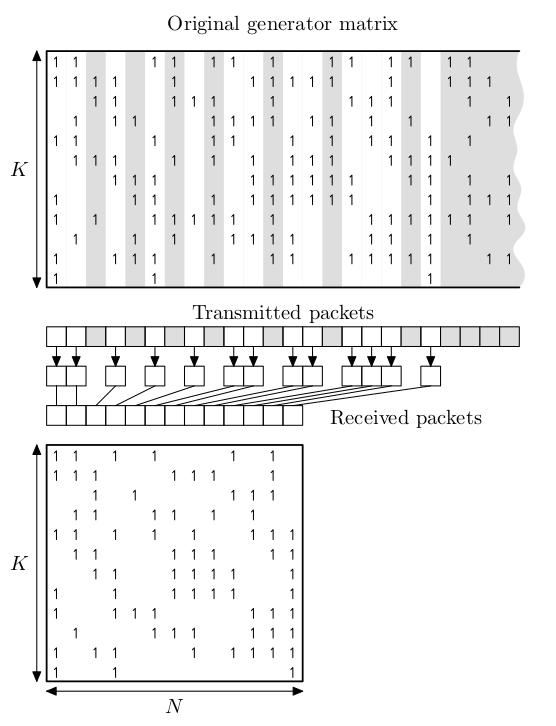
\includegraphics[width=0.4\linewidth]{img/linear_fountain.jpg}
           \end{tabular}
           & \begin{tabular}{l}
             \parbox{0.45\linewidth}{%  change the parbox width as appropiate
             На рисунке слева на белом фоне переданные через канал пакеты,
             на сером -- стертые. \\
             С помощью переданных пакетов (received packets) формируется
             матрица.
    }
    \end{tabular}  \\
    \end{tabular}


\end{frame}

\begin{frame}{Отправляем больше}

    Помним о том, что мы все еще не пользовались избыточностью. 
    Отправим $N=K+E$ пакетов. Тогда вероятность ненахождения
    обратимой подматрицы равномерно ограничена по всем $K$:

    \[
        \delta(E)\le\frac{1}{2^E}
    \]

    \begin{alertblock}{Недостатки}
    
        Обратимую подматрицу нужно
        
        \begin{itemize}
            \item Обратимую подматрицу нужно найти и обратить
            \item Метод плохо масштабируем в силу кубической
            асимптотики
        \end{itemize}
        
    \end{alertblock}

\end{frame}

\subsection{ЛТ-коды}

\begin{frame}{Зачем нам матрицы?}

    \begin{block}{Предложение 1}
        Представим задачу в виде двудольного графа: 
        в одной доле пакеты, в другой -- кодирующие символы.
        
        Отношение связности -- это отношение включения в сумму: то 
        есть символ $s_i$ и пакет $x_j$ смежны
        тогда и только тогда, когда $s_i = x_j\oplus\dots$.
    \end{block}

    \begin{block}{Определение}
        Граф, описанный в предложение 1, называется 
        \textit{графом Таннера}\footnote{\cite{Tanner1981Sep}}.
    \end{block}

    \begin{block}{Предложение 2}
        Последовательно декодируем то, что можем декодировать, и 
        переходим к задаче меньшей размерности.
    \end{block}
    
\end{frame}

\subsubsection{Пример}

\begin{frame}{Лучше показать пример}

    \begin{tabular}{cl}  
         \begin{tabular}{c}
           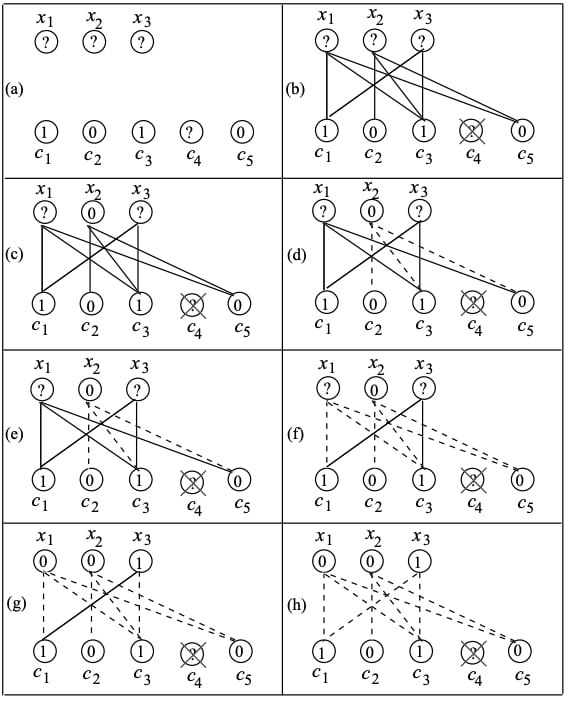
\includegraphics[width=0.4\linewidth]{img/lt_process.jpg}
           \end{tabular}
           & \begin{tabular}{l}
             \parbox{0.47\linewidth}{%  change the parbox width as appropiate
             a) символы $c_1,c_2,c_3,c_5$ прошли через канал \\
             b) визуализируем информацию о связности \\
             c) пакет $x_2$ дошел <<как есть>> в виде символа $c_2$, восстановим его \\
             d) пакет $x_2$ присутствует участвовал в следующих символах:\\
             $c_3 = x_1\oplus x_2\oplus x_3$ и $c_5 = x_1\oplus x_2$ \\
             e) прибавим к обеим частям уравнений выше $x_2$:
             $c_3\oplus x_2=x_1\oplus x_3$, $c_5=x_1$ \\
             f)-h) по тому же алгоритму решаем задачу меньшей размерности          
    }
    \end{tabular}  \\
    \end{tabular}

\end{frame}

\subsubsection{ЛТ-процесс (LT-process, belief propagation)}

\begin{frame}{ЛТ-процесс (LT-process, belief propagation)}

    \begin{block}{Предложение}
        Подберем такой алгоритм генерации символов, чтобы
        ЛТ-процесс завершался успешно с достаточно большой вероятностью.
    \end{block}

    Cхема генерации выглядит так: у нас есть заданное
    распределение степеней символов
    \[
        \boldsymbol{\rho} = (\rho_1,\dots,\rho_K), \:
        \rho_i\ge 0, \:
        \sum_i \rho_i = 1
    \]
    При формировании нового символа из этого распределения сэмплируется
    величина $d$ и для суммирования равновероятно выбираются $d$ из $K$ 
    пакетов:
    \[
        d\sim \boldsymbol{\rho}, \: 
        s_{new} = \sum_{i=1}^d x_{j_i},\:
        j_i\in\{1,\dots,K\},\: s\ne p\Rightarrow j_{s}\ne j_{p}
    \]
\end{frame}

\begin{frame}{Идеальное солитонное распределение}

    \begin{block}{Определение}
        \textbf{Идеальным солитонным распределением} $\boldsymbol{\rho}$
        называется следующий набор чисел:
        \[
            \rho_i=
            \left\{
            \begin{aligned}
                &\frac{1}{K},\: i=1\\
                &\frac{1}{i(i-1)},\: i=2,\dots,K
            \end{aligned}
            \right.
        \]
        Наводящее соображение: на каждом этапе у нас появляется в точности
        один 1 символ.
    \end{block}

    \begin{alertblock}{Недостатки}
        \begin{itemize}
            \item Не работает $\smiley$
            \item Слишком строгое ограничение на процесс
        \end{itemize}
    \end{alertblock}

\end{frame}

\begin{frame}{Робастное солитонное распределение}
    \begin{block}{Определение}
        \textbf{Робастным солитонным распределением} $\boldsymbol{\mu}$
        с параметрами $c>0$ и $0<\delta<1$ называется набор чисел,
        получаемых следующим образом: положим $R=c\ln(K/\delta)\sqrt K$ и
        \[
            \tau_i
            =
            \left\{
            \begin{aligned}
                &\frac{R}{i\cdot K},\: i=1,\dots, \frac{K}{R}-1\\
                &\frac{R\ln(R/\delta)}{K},\: i=\frac{K}{R}\\
                &0,\: i=\frac{K}{R}+1,\dots,k
            \end{aligned}
            \right.
        \]
        Тогда $\mu_i$ -- нормированное $\rho_i+\tau_i$.
    \end{block}
    Наводящее соображение: изменение размера очереди рассматривается 
    как случайное блуждание (стартуем с запасом и используем его, чтобы
    не сломать раньше времени).
\end{frame}

\begin{frame}

    \begin{figure}
    \centering
        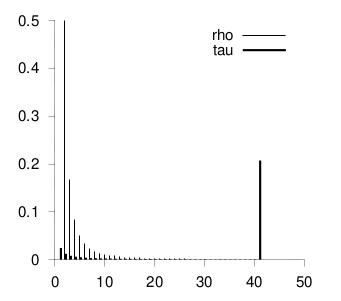
\includegraphics[width=0.4\textwidth]{img/distribution_ex.jpg}
        
        \caption{Пример робастного солитонного распределения, $K=10^4, c=0.2, \delta=0.05$}
        \label{fig:question}
    \end{figure} 

    \begin{block}{Теорема (Лаби, 2002)}
        При получении $K\cdot \sum_{i}(\rho_i+\tau_i)$ символов
        по распределению $\boldsymbol{\mu}_{c,\delta}$ 
        вероятность полного декодирования составляет хотя бы $1-\delta$.
        \footnote{\cite{Luby}}
    \end{block}

\end{frame}

\section{Исследуемая задача}

\subsection{Постановка задачи}

\begin{frame}{Постановка задачи}

    Идея фонтанного кодирования не содержит внутри себя обращения
    к \textbf{порядку} отправки пакетов, поэтому коды работают даже
    если канал передачи информации крайне ненадежен. На практике же
    канал заведомо <<хороший>>, то есть теряет небольшой процент пакетов.
    Используя идеи фонтанного кодирования, будем пытаться сделать хорошего
    канала \textbf{почти идеальный}. 

    \begin{itemize}
        
        \item Процент потерь в канале достаточно мал ($\le5-7\%$) 

        \item Количество пакетов, высылаемых при одних и тех же параметрах,
        невелико (пропускная способность канала зависит от времени)

        \item Коды систематические -- сначала высылаем все <<как есть>>
        
    \end{itemize}

\end{frame}

\subsection{Стратегии исследования}

\begin{frame}{Стратегии исследования}

    Опишем общие стратегии решения. 
    У нас есть 2 степени свободы: алгоритм декодирования $\mathcal D$ и
    распределение $\boldsymbol{\rho}(\cdot)$. 

    \begin{block}{Стратегия 1}

        Использование простого алгоритма декодирования (допускающего аналитический вывод формул)
        и решение задачи условной оптимизации.
        
    \end{block}

    \begin{block}{Стратегия 2}

        Использование сложного алгоритма декодирования (слабо поддающегося анализу)
        и хорошо изученных (Бернулли, Пуассона) или просто устроенных распределений.
    
    \end{block}

\end{frame}

\subsubsection{Стратегия 1}

\begin{frame}{Стратегия 1. Пример простого алгоритма}
    
Пусть имеются пакеты $x_i$, $i=1,\dots, 5$. Отправитель пересылает
через канал их по очереди и до получателя доходят пакеты с номерами
$1, 2, 4$. Далее отправитель пересылает 2 проверочных пакета:
\[s_1 = x_1 \oplus x_2 \oplus x_3\]
\[s_2 = x_1 \oplus x_3 \oplus x_5\]

\begin{itemize}
    \item При получении $s_1$ декодирование будет проведено -- 
    восстановим $x_3$: все пакеты, кроме $x_3$
    -- полученные информационные.
    \item При получении $s_2$ декодирование
    проведено \textbf{не} будет: среди просуммированных пакетов есть 
    два не из списка полученных информационных -- $x_3$ и $x_5$. 
\end{itemize}
 
Данный пример иллюстрирует возможную нерациональность простого алгоритма:
очевидно, что к моменту получения $s_2$ пакет $x_3$ уже восстановлен
и $s_5$ на самом деле восстановить можно.
    
\end{frame}

\begin{frame}{Аналитические формулы}

\[
\mathsf P\{\text{пакет с номером $K$ не будет восстановлен}\} =
\]
\[
=\tau\sum_{I=0}^{K-1}\binom{K - 1}{I}\sum_{C=0}^{M}\binom{M}{C}
\tau^{K - 1 + M - I - C}(1-\tau)^{I + C}\left[
    1 - \sum_{d=1}^{I + 1}\rho_d\frac{\binom{I}{d-1}}{\binom{K}{d}}
\right]^C
\]
\[
=:\tau\cdot \mathcal L(\boldsymbol{\rho}, K, M) 
\]

Получили задачу условной оптимизации:

\[
    \left\{
    \begin{aligned}
        &\mathcal L(\boldsymbol{\rho}, K, M)\to\min\\
        &\rho_i\ge0\\
        &\sum_i \rho_i = 1
    \end{aligned}
    \right.
\]
    
\end{frame}

\begin{frame}{Результаты экспериментов. Метрики}
    \begin{table}[h!]
\begin{center}
    \begin{tabular}{|c|c|c|c|}
        \hline
        $K$ & $M$ & $\tau\mathcal L$, \% & Parity Packet Baseline, \% \\
        \hline
        20 & 2 & 1.23 & 1.32 \\
        \hline
        30 & 2 & 1.54 & 1.76 \\
        \hline
        40 & 2 & 1.78 & 2.09 \\
        \hline 
        20 & 3 & 0.93 & 1.32 \\
        \hline
        30 & 3 & 1.23 & 1.76 \\
        \hline
        40 & 3 & 1.47 & 2.09 \\ 
        \hline
        20 & 4 & 0.74 & 1.32 \\
        \hline 
        30 & 4 & 1.01 & 1.76 \\
        \hline
        40 & 4 & 1.25 & 2.09\\
        \hline
    \end{tabular}
\caption{Результаты экспериментов. $\tau=0.03$}
\end{center}
\end{table}
\end{frame}

\begin{frame}{Результаты экспериментов}
    \begin{figure}
    \centering
    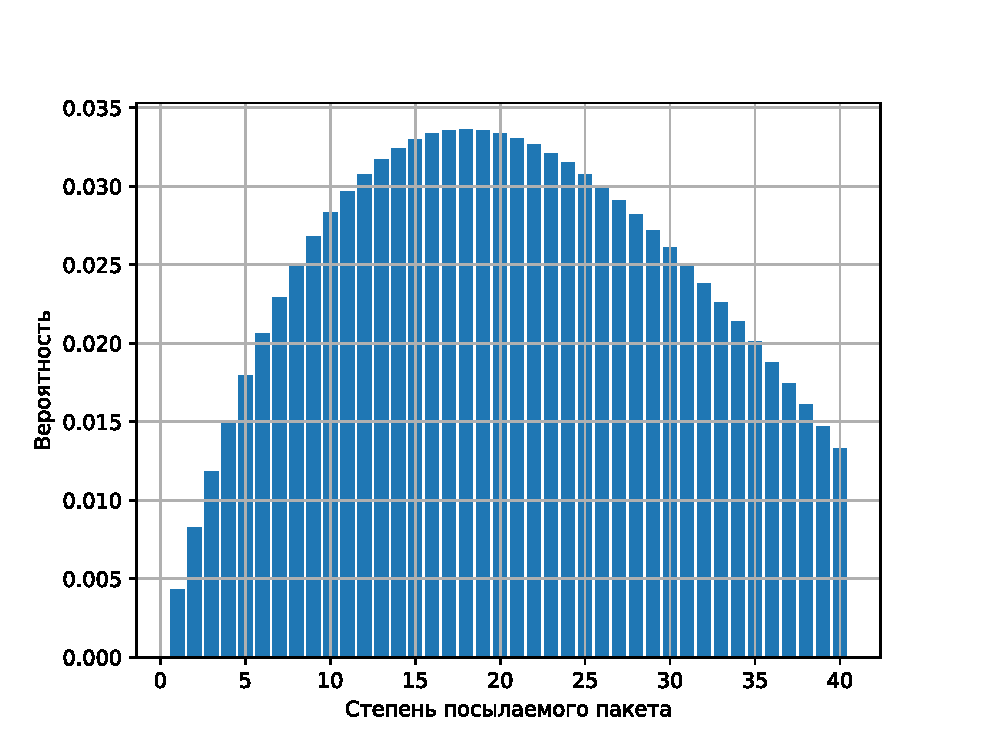
\includegraphics[scale=0.5]{img/distr2.eps}
    \caption{$K=40, \: M=4$}
    %\label{fig:enter-label}
    \end{figure}
\end{frame}

\subsubsection{Стратегия 2}

\begin{frame}{Стратегия 2. Выбор распределений}

    \begin{block}{Наблюдение}
        Хорошо работающие распределения идейно выглядят
        следующим образом: чаще всего генерируются символы одной и
        той же степени, которые постепенно расходуются 
        для поддержания размера очереди.
    \end{block}

    Таким условиям удовлетворяют биномиальное и Пуассоновские распределения,
    а также, например:
    \[
        \rho_i=
        \left\{
        \begin{aligned}
            &1,\: i = d\\
            &0,\: i\ne d
        \end{aligned}
        \right.
    \]
    Рассмотрим их подробнее.
    
\end{frame}

\begin{frame}{Биномиальное распределение}
    

    \begin{table}[h!]
    \begin{center}
        \begin{tabular}{|c|c|c|c|c|}
            \hline
            $K$ & $N$ & $p_{\text{опт}}$ & $p_{BEC}$ & $\tau$ \\ 
            \hline
            20 & 24 & 0.571 & 0.05 & 0.01 \\
            \hline
            20 & 24 & 0.776 & 0.03 & 0.003 \\ 
            \hline 
            50 & 60 & 0.286 & 0.05 & 0.008 \\ 
            \hline
            50 & 60 & 0.327 & 0.03 & 0.002 \\
            \hline
        \end{tabular}
    \caption{Результаты экспериментов. Избыточность 20\%}
    \end{center}
    \end{table}
\end{frame}

\begin{frame}{Пуассоновское распределение}
    \begin{table}[h!]
    \begin{center}
        \begin{tabular}{|c|c|c|c|c|}
            \hline
            $K$ & $N$ & $\lambda_{\text{опт}}$ & $p_{BEC}$ & $\tau$ \\ 
            \hline
            20 & 24 & 10.6 & 0.05 & 0.01 \\
            \hline
            20 & 24 & 11.0 & 0.03 & 0.004 \\ 
            \hline 
            50 & 60 & 15.3 & 0.05 & 0.007 \\ 
            \hline
            50 & 60 & 18.6 & 0.03 & 0.001 \\
            \hline
        \end{tabular}
    \caption{Результаты экспериментов. Избыточность 20\%}
    \end{center}
    \end{table}
\end{frame}


\section{Направления дальнейший исследований}

\begin{frame}{Направления дальнейших исследований}

    \begin{itemize}
        \item Исследование дисперсии числа восстановленных пакетов
        \item Поиск способов точного вычисления вероятностей восстановления
        \item Изучение решений оптимизационной задачи из стратегии 1
    \end{itemize}
    
\end{frame}

\end{document}
